\documentclass[12pt,a4paper]{ctexart}
\usepackage{amsmath,amsthm,amssymb,appendix,bm,graphicx,hyperref,mathrsfs,abstract,geometry,cite}

\title{\textbf{圆周率的探索史和计算方法的研究}}
\author{自动化2211班~~陈博 U202214123}
\date{}%日期(这里避免生成日期,具体看个人需求)
\linespread{1.5}

%%定理环境
\geometry{a4paper, left=3cm, right=3cm, top=1.5cm, bottom=1.5cm}

\newtheorem{theorem}{定理}[section]
\newtheorem{definition}[theorem]{定义}
\newtheorem{lemma}[theorem]{引理}		
\newtheorem{corollary}[theorem]{推论}
\newtheorem{example}[theorem]{例}
\newtheorem{proposition}[theorem]{命题}
%%
\renewcommand{\abstractname}{\Large\textbf{摘要}}

\begin{document}
	\maketitle
	\setcounter{page}{0}
	\maketitle
	\thispagestyle{empty}
	
	\begin{abstract}
		圆,生活中处处可见的事物,而与之密不可分的圆周率,即$\pi$,平日里我们经常和它打交道,一些公式、定理中也能见到它的身影。但是,在使用它的时候,我未曾想过这个神奇的数字是怎么来的,未曾思考过它是如何被计算出来的,并且精确度还能不断提高……解决这些问题,不仅可以让我们通过数学史来感受数学的美好,而且能够一定程度上提高我们的数学能力,拓展我们的思维。本文通过查阅各种资料和推演部分公式,来进行对圆周率的研究。通过本次探索,我们发现圆周率的计算,是一个逐步精确的艰难过程,体现在方法的优化,计算手段的优化等方面。圆周率的计算史,侧面反映了数学的进步史,是一个艰苦且浪漫的过程。
		\\\textbf{关键词:}圆周率,数学史,级数,弹性碰撞,割圆法
	\end{abstract}
	
	%\newpage
	\setcounter{page}{1}
	\pagenumbering{arabic}
	\section{前言}
	在对自然界的认识上,直线和圆大概是人最早引起注意的几何图形。其中圆的图形,容易从太阳、满月、向日葵的花盘、一些花的形状,以及水面的涟漪上体会到。另一方面,人们对于周期性变化的事物较有兴趣,亚里士多德说“圆运动先于直线运动,因为它比较单一”,“循环运动是一切运动的尺度”。圆形的轮子是人类历史上最重要的发明之一,由其衍生出来的齿轮在工业革命中起到了无法代替的作用\cite{RN22}。
	
	对于圆,人们开始注意圆的直径D决定了其大小,同样也会注意到圆的周长C,并逐步加深了对二者之间关系的认识。经过很长一段时间,才会认识到周长与直径成正比,而这一比值,就是圆周率。
	
	但是对于圆周率,我们如今在使用它的时候,很少去思考为什么圆周率是这个值,圆周率是怎么样被定义和被算出来的,圆周率的计算史到底是怎么样的。解决这些问题,不仅可以让我们感叹于数学史的坎坷与浪漫,与数学家们进行跨时空的“对话”,而且能够一定程度上拓展我们的思维、提高我们的数学能力。
	
	1736年,瑞士数学家欧拉提倡以希腊字母$\pi$来表示圆周率, 是圆周的希腊文的字头。欧拉的建议后来逐渐为大家接受。直到现在,$\pi$已成为圆周率的专用符号。
	
	圆周率的计算最早可以追溯到公元前20世纪,一块古巴比伦石匾清楚地记载了圆周率的值。埃及人似乎在更早的时候就知道圆周率了。英国作家John Taylor在其名著《金字塔》中指出,造于公元前2500年左右的胡夫金字塔和圆周率有关,即金字塔的周长和高度之比等于圆周率的两倍,正好等于圆的周长和半径之比。
	
	一直到今天,圆周率的计算方法经历了实验法、几何法、分析法和电脑计算这几个过程,全国各地都有数学家们都为圆周率的计算付出了很大的努力\cite{RN21}。从以前的割圆法,到利用微积分来计算圆周率\cite{RN20},以及可能用一维弹性碰撞来计算圆周率\cite{RN23},方法非常的多。
	
	研究圆周率的计算史,掌握一些计算圆周率的方法,一定程度上可以帮助拓展我们的思维,对数学有一个更深刻的理解。
	\section{材料与方法}
	\subsection{圆周率的探索史}
	\subsubsection{几何法时期}
	古希腊作为古代几何王国对圆周率的贡献尤为突出。古希腊大数学家阿基米德开创了人类历史上通过理论计算圆周率近似值的先河。阿基米德从单位圆出发,先用圆内接正六边形求出圆周率的下界为3,再用外接正六边形并借助勾股定理求出圆周率的上界小于4。接着,他对圆内接正六边形和圆外接正六边形的边数分别加倍,将它们分别变成内接正12边形和外接正12边形,再借助勾股定理改进圆周率的下界和上界。他逐步对内接正多边形和外接正多边形的边数加倍,直到内接正96边形和外接正96边形为止。最后,他求出圆周率的下界和上界分别为223/71和22/7,并取它们的平均值3.141851为圆周率的近似值。阿基米德用到了迭代算法和两侧数值逼近的概念,称得上是“计算数学”的鼻祖\cite{RN21}。
	
	《周髀算经》的中有“径一而周三”的记载,意即$\pi=3$。汉朝时,张衡得出3.162的结果。这个值不太准确,但它简单易理解。
	
	公元263年,中国数学家刘徽用“割圆术”计算圆周率,他先从圆内接正六边形,逐次分割一直算到圆内接正192边形。他说:“割之弥细,所失弥少,割之又割,以至于不可割,则与圆周合体而无所失矣。”这包含了求极限的思想。刘徽给出$\pi=3,141024$的圆周率近似值,刘徽在得圆周率=3.14之后,发现3.14这个数值还是偏小。于是继续割圆到1536边形,求出3072边形的面积,得到令自己满意的圆周率\cite{RN21}。
	
	祖冲之,字文远,范阳郡遒县(今河北省保定市涞水县)人,是我国南北朝时期著名数学家、天文学家。祖冲之关于圆周率有两大贡献:其一是求得圆周率:$3.1415926<\pi<3.1415927$;其二是得到$\pi$的两个近似分数:约率为22/7;密率为355/113。
	
	祖冲之曾写过一本数学著作《缀术》,记录了他对圆周率的研究和成果。但当时“学官莫能究其深奥,是故废而不理”,以致后来失传。很多人都知道用密率355/113表示$\pi$的近似值,是一项了不起的贡献。密率355/113传到了日本后,日本数学史家三上一夫1913年建议将祖冲之圆周率的密率数值命名为“祖率”,得到大家一致赞同。祖冲之对圆周率的求索,超过了世界水平整整1000年!直到16世纪德国人V·奥托才发现了圆周率的密率355/113。但是“祖率”的妙处和给今人留下的困惑,不少人却说不出来。
	
	祖率(密率)是圆周率十分精确的近似值,且又很好记。张景中院士在《数学家的眼光》一书中指出:它与$\pi$精确值的误差不超过0.000000267。在数学家看来,好的近似分数,既要精确,分母最好又不太大。现今数学上已不难证明,在所有分母不超过16500的分数中,密率355/113是当之无愧的冠军。因为《缀术》失传了,祖冲之究竟是用什么方法将$\pi$算到小数点后第7位,又是怎样找到既精确又方便的密率的呢?这至今仍是困惑数学家的一个谜。在中国科协2008年3月13日出版的《科技导报》杂志的第26卷第5期《18个中国公众关注的科技问题》一文中,己将“祖冲之究竟是怎样计算出圆周率$\pi$值的?”列为公众关注的未解科学难题之一\cite{RN21}。
	
	在之后的800年里祖冲之计算出的$\pi$值都是最准确的。
	
	约在公元530年,印度数学大师阿耶波多算出圆周率约为。婆罗摩笈多采用另一套方法,推论出圆周率等于10的算术平方根。
	
	阿拉伯数学家卡西在15世纪初求得圆周率17位精确小数值,打破祖冲之保持近千年的纪录。德国数学家鲁道夫·范·科伊伦于1596年将$\pi$值算到20位小数值,后投入毕生精力,于1610年算到小数后35位数,该数值被用他的名字称为鲁道夫数。
	\subsubsection{分析法时期}
	这一时期人们开始利用无穷级数或无穷连乘积求$\pi$,摆脱可割圆术的繁复计算。无穷乘积式、无穷连分数、无穷级数等各种π值表达式纷纷出现,使得值计算精度迅速增加。
	
	第一个快速算法由英国数学家梅钦提出,1706年梅钦计算值突破100位小数大关,他利用了如下公式:\begin{equation}\pi/4=4\arctan1/5-\arctan1/239,\end{equation}其中$\arctan{x}$可由泰勒级数算出。类似方法称为“梅钦类公式”。
	
	到1948年英国的弗格森和美国的伦奇共同发表了$\pi$的808位小数值,成为人工计算圆周率值的最高纪录\cite{RN21}。
	\subsubsection{计算机时期}
	电子计算机的出现使$\pi$值计算有了突飞猛进的发展。1949年,美国制造的世上首部电脑——ENIAC在阿伯丁试验场启用了。次年,里特韦斯纳、冯纽曼和梅卓普利斯利用这部电脑,计算出$\pi$的2037个小数位。五年后,IBMNORC只用了13分钟,就算出$\pi$的3089个小数位。在1973年,电脑CDC 7600发现了$\pi$的第一百万个小数位。
	
	1989年美国哥伦比亚大学研究人员用克雷-2型(Cray-2)和IBM-3090/VF型巨型电子计算机计算出$\pi$值小数点后4.8亿位数,后又继续算到小数点后10.1亿位数。2010年1月7日——法国工程师法布里斯·贝拉将圆周率算到小数点后27000亿位。2010年8月30日——日本计算机奇才近藤茂利用家用计算机和云计算相结合,计算出圆周率到小数点后5万亿位\cite{RN21}。
	
	2011年10月16日,日本长野县饭田市公司职员近藤茂利用家中电脑将圆周率计算到小数点后10万亿位,刷新了2010年8月由他自己创下的5万亿位吉尼斯世界纪录。56岁的近藤茂使用的是自己组装的计算机,从10月起开始计算,花费约一年时间刷新了纪录\cite{RN21}。
	\subsection{圆周率的计算方法}
	\subsubsection{微积分}
	在大一下学期,我学习了无穷级数,里面有一些级数收敛于与圆周率有关的结果,因此,通过查阅资料后,我发现了通过无穷级数来计算圆周率的可能性,下面是简单的计算过程。
	
	首先,对于幂级数,它的定义是这样的:
	\begin{equation}{{a}_{0}}+{{a}_{1}}x+{{a}_{2}}{{x}^{2}}\cdots +{{a}_{n}}{{x}^{n}}+\cdots =\sum\limits_{n=0}^{\infty }{{{a}_{n}}{{x}^{n}}},\end{equation}
	其中,$a_n$为系数,$x$为自变量,一旦幂级数中所有系数和自变量的值被确定,我们很容易计算前有限项的值作为该幂级数的近似值。因此,为了计算一个给定的函数 ,我们经常把它转化成一个简单的幂级数来计算该函数的近似值。这个通过 转化成的简单幂级数也被称为函数 的麦克老林级数,记为:
	\begin{equation}\label{simple_equation}f(x)\sim f(0)+\frac{{f}'(0)}{1!}x+\frac{{f}''(0)}{2!}{{x}^{2}}+\cdots +\frac{{{f}^{(n)}}(0)}{n!}{{x}^{n}}+\cdots,\end{equation}
	通过指定$f(x)$和$x$,即可计算圆周率的值。
	
	在公式\ref{simple_equation}中,令$f(x)=\arctan{x}$和$x=1$,我们可以得到如下公式:
	\begin{equation}\frac{\pi }{4}=1-\frac{1}{3}+\frac{1}{5}+\cdots +{{(-1)}^{n}}\frac{1}{2n+1}+\cdots ,\end{equation}
	利用它来计算圆周率是非常方便的。
	
	不仅如此,利用不同的函数和不同的$x$的值,通过幂级数和傅里叶级数可以得到很多与圆周率有关的公式:
	\begin{equation}\frac{{{\pi }^{2}}}{6}=1+\frac{1}{{{2}^{2}}}+\frac{1}{{{3}^{2}}}+\cdots +\frac{1}{{{(2n-1)}^{2}}}+\cdots ,\end{equation}
	以及
	\begin{equation}\frac{{{\pi }^{2}}}{8}=1+\frac{1}{{{3}^{2}}}+\frac{1}{{{5}^{2}}}+\cdots +\frac{1}{{{(2n-1)}^{2}}}+\cdots ,\end{equation}
	它们都可以被用来计算圆周率\cite{RN20}。
	\subsubsection{矩阵与一维弹性碰撞}
	在靠光滑竖直墙壁的光滑水平面上放置一个质量为$m_1$的弹性滑块,在滑块$m_1$与光滑竖直墙壁之间另放置一个质量为$m_2$的弹性滑块.现给$m_1$一个水平向左的初速度,$m_1$与$m_2$之间会发生若干次弹性碰撞,如果$m_1$是$m_2$质量的1倍、100倍、10000倍、1000000倍、100000000倍……那么总碰撞次数分别为3、31、314、3141、31415……也就是说,一维完全弹性碰撞次数蕴涵着圆周率\cite{RN23}。
	
	不失一般性,假定两个弹性滑块的质量$m_1$、$m_2$之间满足$m_1=km_2$,其中$k>0$。设初始状态 $m_1$、$m_2$的初速度分别为$u_0$、$v_0$,$m_1$、$m_1$间第$n+1$次碰撞前的速度分别为$u_n$、$v_n$,如图\ref{fig:一般化碰撞模型}所示。
	\begin{figure}[htbp]
		\centering
		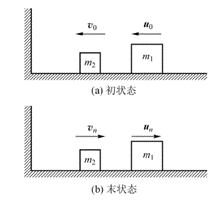
\includegraphics{一般化碰撞模型.png}
		\caption{一般化碰撞模型}
		\label{fig:一般化碰撞模型}
	\end{figure}
	
	通过计算,我们首先可以得到第一次碰撞后两滑块的速度:
	\begin{equation}{{u}_{1}}=\frac{k-1}{k+1}{{u}_{0}}+\frac{2}{k+1}{{v}_{0}},\end{equation}
	\begin{equation}{{v}_{1}}=\frac{-2k}{k+1}{{u}_{0}}+\frac{k-1}{k+1}{{v}_{0}},\end{equation}
	连续的碰撞可以看作速度的变换,利用线性代数的知识,我们可以得到$m_1$、$m_2$第$n+1$次碰撞前速度的三角函数形式表达式:
	连续的碰撞可以看作速度的变换,利用线性代数的知识,我们可以得到 、 第 次碰撞前速度的三角函数形式表达式:
	\begin{equation}{{u}_{n}}={{u}_{0}}\cos n\theta +{{v}_{0}}\frac{\sin n\theta }{\sqrt{k}},\end{equation}
	\begin{equation}{{v}_{n}}=-{{u}_{0}}\sqrt{k}\sin n\theta +{{v}_{0}}\cos n\theta ,\end{equation}
	其中$\theta$的满足$\theta =arccos\frac{k-1}{k+1}$。
	
	当$m_2$初始状态静止时,我们最终可以得到如下关系:
	\begin{equation}\label{公式11}\frac{{{N}_{1}}}{\sqrt{k}}\approx \pi ,\end{equation}
	公式\ref{公式11}揭示了碰撞次数$N_1$与$\sqrt{k}$之间的紧密联系,利用此关系可以测出$\pi$的数值。
	
	当$m_2$初始状态静止时,我们最终可以得到如下关系:
	\begin{equation}\label{公式12}\frac{2{{N}_{2}}}{\sqrt{k}}\approx \pi ,\end{equation}
	公式\ref{公式12}揭示了碰撞次数$N_2$与$\sqrt{k}$之间的紧密联系,利用此关系可以测出$\pi$的数值,部分数据如表\ref{table1}所示\cite{RN23}。	
	
	\begin{table}[h]
		\caption{ $k=1\times {{10}^{2s}}(s=0,1,2,3\cdots )$时,对应$N_1$,$\frac{{{N}_{1}}}{\sqrt{k}}$,$N_2$,$\frac{2{{N}_{2}}}{\sqrt{k}}$的数值}
		\centering
		\begin{tabular*}{\hsize}{@{\extracolsep{\fill}}c c c c c}
			\hline
			$k$ & $N_1$ & $\frac{{{N}_{1}}}{\sqrt{k}}$ & $N_2$ & $\frac{2{{N}_{2}}}{\sqrt{k}}$ \\
			\hline
			$1\times {{10}^{0}}$ & 3 & 3 & 1 & 2\\
			$1\times {{10}^{2}}$ & 31 & 31  & 15 & 3.0\\
			$1\times {{10}^{4}}$ & 314 & 314  & 157  & 3.14\\
			$1\times {{10}^{6}}$ & 3141 & 3141  & 1570  & 3.140\\
			$1\times {{10}^{8}}$ & 31415 & 31415  & 15707  & 3.1414\\
			$1\times {{10}^{10}}$ & 314159 & 314159  & 157079 & 3.14158\\
			$1\times {{10}^{12}}$ & 3141592 & 3141592  & 1570796 & 3.141592\\
			$1\times {{10}^{14}}$ & 31415926 & 31415926  & 15707963 & 3.1415926\\
			$1\times {{10}^{16}}$ & 314159265 & 314159265  & 157079632  & 3.14159264\\
			$1\times {{10}^{18}}$ & 3141592653 & 3141592653  & 1570796326  & 3.141592652\\
			$1\times {{10}^{20}}$ & 31415926535 & 31415926535  & 15707963267  & 3.1415926534\\
			\hline
		\end{tabular*}
		\label{table1}
	\end{table}
	
	
	\section{讨论}
	圆周率的探索史,是一部艰苦浪漫的探索史,古今中外,很多数学家为了计算圆周率的值付出了不可估量的努力。实际上3.1416一般情况下己够用了,这样的计算并没有什么实际上的需要。但究竟是什么原因推动了这种对$\pi$的计算狂热呢?
	
	从积极方面看,大致的理由是:
	
	(1)计算$\pi$有各种计算方法,采用同一台计算机,可以比较哪种方法能用较少的工作量算出更高精度的$\pi$值。
	
	(2)采用同一种计算 的方法,对不同的计算机的能力也是一个比较和考验。
	
	(3)希望算出$\pi$在小数点后更多的数值来观察和研究$\pi$的性质。如$\pi$是有理数,则是一个有限小数,或无限循环小数;如$\pi$是无理数,就是无限不循环小数。大量的计算可看出些端倪,给进一步的严格证明提供启示。
	
	当然也有希望创记录、一举成名的心理因素。以往也常有死背$\pi$很多位值的事,以锻炼记忆力。其实这对于圆周率$\pi$的研究,己无多大意义。
	
	那么 具有哪些性质呢?1767年,兰伯特证明了$\pi$是无理数。1775年,欧拉又提出问题: $\pi$会不会是一个整系数代数方程的根,即是一个代数数呢?如果不是代数数,就称为超越数。1882年,林德曼在欧拉提出问题的107年后,证明了$\pi$是一个超越数。从人类对圆周率$\pi$的认识不断深化的历史,可以看出科学是充满活力并不断开拓前进的\cite{RN21}!
	
	对于计算圆周率的方法,目前我学过的就有级数这一重要方法,相信还有更多更好的方法能够计算出$\pi$的值。与此同时,物理中,我们或许可以找到二维弹性碰撞与圆周率的关系,未来圆周率的计算一定能再上升一个高度。
		
	\section{总结}	
	本文介绍了圆周率的探索史,圆周率$\pi$是一个神奇的事物,让我无比感慨于数学的美妙与神奇。
	
	古今中外,很多数学家都为圆周率的计算出了一份力,其中,我国的数学家祖冲之,对圆周率计算的贡献度非常高,华罗庚先生在1964年曾说:“祖冲之虽已去世一千四百多年,但他的广泛吸收古人成就而不为其所拘泥、艰苦劳动、勇于创造和敢于坚持真理的精神,仍旧是我们应当学习的榜样”。1967年11月9日紫金山天文台将1964年发现的小行星1888(1964 VO1)命名为祖冲之小行星。1967年国际天文学家联合会将月球上的一座环形山命名为“祖冲之环形山”。为纪念祖冲之这位祖藉河北保定的科学家,在他的故乡河北保定市,河北大学1986年9月9日在图书馆的大门前,建立了祖冲之塑像。
	
	祖冲之是中华民族的骄傲,也是当今创新研究和发展的榜样。
	
	对于计算圆周率,本文提出了两种方法,一种是级数,一种是一维弹性碰撞,对于圆周率的计算方法,还有很多很多,圆周率的计算,未来一定能提升到一个新高度!
	
	\bibliographystyle{plain}
	\bibliography{MyEndNoteLibrary}
\end{document} 
